\section{Architektur}

\begin{figure}[ht]
	\centering
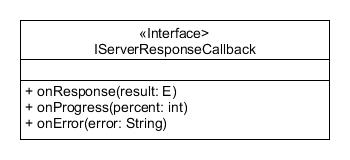
\includegraphics[width=1\textwidth]{./resources/Diagramme/App/UMLAndroidApp.jpg}
\caption{UML Diagram der Android App}
	\label{fig:modules_overview}
\end{figure}

\subsection{Entwurfsmuster}
In der App werden Entwurfsmuster verwendet, um Komponenten leicht austauschen zu können und um die Nutzeroberfläche und den Funktionsumfang einfach erweitern zu können. Der Einsatz von Entwurfsmustern Verhindert  zudem, dass Klassen über Schichten hinweg Zugriff haben und reduziert die Aufrufe von Klassen einer niederen Schicht auf die darüber liegende Schicht. Sie helfen ferner bei der Enkopplung einzelner Komponenten voneinander und unterstützen das Geheimnisprinzip.

\subsubsection{Decorator}
Das Decorator Muster wird bei der Klasse \nameref{app:klasse:TriggeringCompatCameraHandler} angewendet. Diese dekoriert die Klasse \nameref{app:klasse:CompatCameraHandler}, indem er von dieser erbt und in seinem Konstruktor einen \textit{super} Aufruf tätigt, um den Konstruktor der Elternklasse aufzurufen. Der Decorator delegiert jeden Methodenaufruf an seine Elternklasse, fügt aber Funktionen zum Behandeln von Klick-Events und dem Überwachen des G-Sensors hinzu.
Dadurch wird die Funktion des CompatCameraHandlers erweitert, ohne dass er davon wissen muss.

\subsubsection{Observer}
Das Observer Muster reduziert die Aufrufe von Klassen einer niederen Schicht auf die darüber liegende Schicht. In der App gibt es die Observer \nameref{app:klasse:IRecordCallback}, das \nameref{app:klasse:IPersistCallback} und das \nameref{app:klasse:IServerResponseCallback}. Nützlich ist das Observer Muster vor allem dann, wenn ein asynchroner Task ausgeführt wird und der Aufrufer erst benachrichtigt werden soll, wenn dieser Task zu Ende ist.\newline
Bei der Umsetzung des Observer Musters weicht die App von der herkömmlichen Art ab: Während normalerweise eine Klasse, die als Observer agiert, das Interface, also einen der Callbacks, implementiert, hat in der App im Gegensatz dazu eine Klasse ein Attribut vom Typ des jeweiligen Interfaces. Bei der Instanziierung dieses Attributes findet die Implementierung des Interfaces statt.

\subsubsection{Command}
Das Command Muster kommt bei jedem asynchronen Task zum Einsatz. Er ermöglicht die Abkopplung der Hintergrundprozesse von den Vordergrundprozessen. Somit kann der Aufrufer direkt mit seinen Aufgaben fortfahen, während der Command im Hintergrund ausgeführt wird. Sobald er seine Aufgaben beented hat wird der Empfänger des Commands benachrichtigt und kann damit beginnen, das Resultat des Commands zu verarbeiten.\newline
In den Konstruktoren der Commands werden diese parametrisiert, durch die \textit{start} Methode wird der Command ausgeführt. Der \nameref{app:klasse:AuthenticateTask} authentifiziert den Nutzer, indem er auf das Netzwerk zurückgreift. Ebenso greift der \nameref{app:klasse:VideoUploadTask} auf das Netzwerk zu um ein Video hochzuladen. Der \nameref{app:klasse:AsyncPersistor} speichert ein Video asynchron ab. Jeder dieser Commands erhält in seinem Konstruktor und durch die \textit{start} Methode alle Daten, die er zur Ausführung benötigt. Das Callback, welches jeder Command übergeben bekommt, dient als Empfänger, die Rolle des Invokers und des Klientens werden beide von der Klasse übernommen, die den Command instanziiert.

\subsubsection{Proxy}
Das Proxy Muster kommt zum Einsatz, sobald Anfragen an den Server gesendet werden oder Operationen auf dem Speicher ausgeführt werden sollen. Die entsprechenden Klassen sind \nameref{app:klasse:ServerProxy} und \nameref{app:klasse:MemoryManager}. Dadurch muss keine der Klassen, die den ServerProxy oder den MemoryManager verwenden, über die zugrunde liegende Infrastruktur und deren Handhabung Bescheid wissen.

\subsubsection{Template Method}
Das Template Method Muster, zu Deutsch ``Schablonenmethode'', findet seinen Einsatz in der \nameref{app:klasse:ContainerActivity}. Die ContainerActivity ist eine Activity, die immer nach dem gleichen Schema aufgebaut ist: Eine Toolbar am oberen Bildschirmrand und ein Fragment mit dem Inhalt darunter. Sie selbst lädt immer die gleiche Ansicht, lässt aber ihre Unterklasse bestimmen, welches Fragment angezeigt wird. Dadurch können ohne großen Aufwand weitere Ansichten eingefügt werden. Der einzige Aufwand besteht im Erben von ContainerActivity und dem Implementieren der \textit{selectFragment} Methode.\newline
Sollte später eine Activity mit einem ViewPager eingefügt werden, der beispielsweise aufgenommene und heruntergeladene Videos in eigenen Tabs anzeigen kann, bietet sich die Schablonenmethode wieder an: In diesem Fall gibt es eine Acitivty, die ein Layout lädt, das über einen ViewPager verfügt. Die Unterklassen bestimmen dann auf welcher Seite welches Fragment eingeblendet wird. Natürlich muss die Nummer des aktuellen Tabs des ViewPagers in der \textit{selectFragment} Methode mitgeliefert werden.

\subsubsection{Strategy}
Die Strategy Methode kommt in den Klassen \nameref{app:klasse:CameraHandler}, \nameref{app:klasse:IFileEncryptor} und \nameref{app:klasse:IKeyEncryptor}  zum Einsatz. Sie ermöglicht die Austauschbarkeit der Kameraimplementierung bzw. der Verschlüsselungsalgorithmen und macht ihre Klienten nur von den Schnittstellen abhängig.
\newpage
